\documentclass[a4paper,ngerman]{scrartcl}

\usepackage{amsmath}
\usepackage{amsfonts}
\usepackage{amssymb}
\usepackage[utf8]{inputenc}
\usepackage{graphicx}
\usepackage[ngerman]{babel}
\usepackage{hyperref}
\usepackage{float}
\usepackage{caption}
\usepackage{subcaption}
\usepackage{multirow}  %for tables
\usepackage{icomma} % Handle german comma as decimal point in numbers
\usepackage{units,siunitx} % Write units with correct spacing
\usepackage{upgreek} % provide non-italic greek letters
\usepackage{url}
%\usepackage{subfig}

% Formatting of table & figure captions
\captionsetup{font={sf,footnotesize},labelfont=bf,textfont=sl,skip=6pt}
\setlength{\abovecaptionskip}{6pt}
\setlength{\belowcaptionskip}{0pt}

\title{Black Lipid Membrane\\ Auswertung}
\date{\today}
\author{Michel Rausch, Michael Eliachevitch}

\begin{document}

\maketitle
\tableofcontents
\newpage

\section{Aufgabe 1: Vorbereitung der Lipidmembran}

\section{Aufgabe 2: Messung einzelner Ionenkanäle}

\section{Aufgabe 3: Messung multipler Ionenkanäle}

In Aufgabe 2 sind bereits mehrere Kanäle beobachtet worden. Die gesamte Spritze wurde entleert, sodass sich 1 ml Gramicidin A in der Lösung befanden. Unter diesen Bedingungen war es noch schwieriger eine stabile Lipidschicht aufzubauen.
Die Schicht platzte nach kurzer Zeit, insbesondere nach Anlegen einer Spannung, sodass die Messung nur in einem Intervall von einer Minute erfolgen konnte.

Es ist ein Rauschen zu erkennen, bei dem 

\begin{figure}
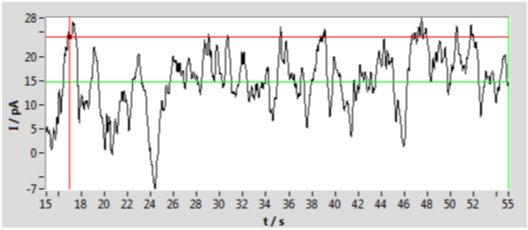
\includegraphics[width=0.8\textwidth]{abbildungen/mehrkanal_raw.png}
\caption{Strom durch eine Lipidmembran bei einer hohen Konzentration von Gramicidin A}
\label{fig:mehrkanal-roh}
\end{figure}


\begin{figure}
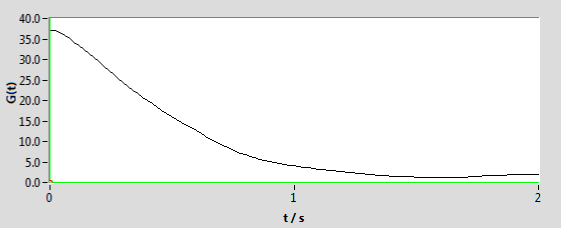
\includegraphics[width=0.8\textwidth]{abbildungen/mehrkanal_korrel.png}
\caption{Autokorrelationsfunktion der Messungen aus Abbildung \ref{fig:mehrkanal-roh}}
\label{fig:mehrkanal-korrel}
\end{figure}


\section{Aufgabe 4: Weitere Fragen}

\section{Quellen}
\begin{enumerate}
\item Vorbereitungsmappe 
\end{enumerate}



\end{document}
